% Introduction

\chapter{Introduction}

Embedded systems are specialized computer systems that are designed to perform specific tasks or
functions within a larger system. They are integral to a wide variety of devices and applications,
enabling seamless functionality and efficiency in our daily lives. These systems tightly integrate
hardware and software components to optimize performance, power consumption, and system size.
The importance of embedded systems lies in their ubiquity and versatility. They can be found in
numerous devices and industries, including consumer electronics, telecommunications, automotive,
aerospace, medical, and industrial automation. Examples of embedded systems include microcontrollers
in smart home appliances, digital signal processors in wireless communication devices, control systems
in autonomous vehicles, and sensor networks for monitoring and automation\cite{marwedel2021embedded}.

As the world becomes increasingly interconnected and reliant on technology, the role of embedded
systems continues to expand. They are essential for enabling the \acrlong{iot}, as well as
advancements in artificial intelligence, robotics, medical instruments, and
smart cities\cite{camposano1996embedded:ARTICLE}. As of February 2023, there are an estimated
21.5 billion interconnected devices in the world, according to
Statistas\cite{IoTconne16:online}\cite{HowManyI1:online}.
This number is expected to continue to increase as internet consumption rises and
new gadgets and machinery are introduced to the market and by 2025,
it is projected that 75.44 billion IoT devices will be installed worldwide\cite{HowManyI1:online}.

The number of embedded devices per person is significantly higher in developed
countries than in developing nations. For example, in the United States, there
were approximately 13 IoT devices per person in 2020\cite{Stateoft48:online}.
In comparison, the global average was around 3.5 IoT devices per person during
the same year\cite{CiscoAnn1:online}. In developed countries, prevalent devices
typically include intelligent home appliances, wearable technology, and interconnected vehicles.
Whereas, a greater concentration of devices aimed at supporting agriculture, healthcare, and monitoring
critical infrastructure in developing countries. The most common smart home devices include smart
thermostats, smart lighting, smart security systems, and smart appliances like refrigerators and washing machines.
The fitness trackers, smartwatches, and health monitoring devices. Sensors are used for soil
monitoring and as agricultural devices.

The exponential growth of embedded systems necessitates robust security, reliability, and
efficiency measures to ensure the safety and functionality of the technology we rely on daily\cite{muench2018you}.
Mirai malware attacks have demonstrated their potential for large-scale disruption, targeting
devices like routers, cameras, and DVRs to execute \gls{DDoS} attacks.
In 2016, a \gls{ddos} attack on Dyn, a DNS provider, significantly hindered user access to prominent
services such as Twitter, Amazon, Tumblr, Reddit, Spotify, and
Netflix\cite{muench2018you}\cite{lindqvist2017future}. \textit{Ripple20},
a set of 19 critical vulnerabilities in the Treck TCP/IP library,
impacted IoT devices used in industrial control systems, healthcare devices,
and home appliances. URGENT/11 and BadAlloc, discovered in the VxWorks \gls{RTOS},
affected millions of embedded devices, including medical devices, industrial control systems,
and routers\cite{seri2019critical}. These vulnerabilities originate from memory allocation functions
and can lead to remote code execution, allowing attackers to seize control of compromised devices.

Software testing is a critical process in the development of embedded systems,
where the software is evaluated to verify that it meets the specified requirements,
functions as intended, and is free from defects or vulnerabilities. The primary benefits of
software testing include improved software quality, increased reliability, enhanced security,
and reduced development costs and time-to-market\cite{819971}. Traditional testing methods,
including manual and automated testing, have been the standard approach.
However, these methods have limitations in uncovering all potential vulnerabilities and edge cases, particularly in the context of
software security. As the consequences of security breaches discussed above, it becomes increasingly severe,
there is a pressing need for the company to explore and adopt more
advanced testing techniques that can address security related challenges more effectively.

Fuzz testing, also known as fuzzing, is a powerful and popular technique for testing software
applications, and it has proven particularly effective in identifying security vulnerabilities.
Fuzz testing involves dynamically generating input data variations based on valid seeds,
enabling the exploration of edge cases and the detection of bugs that are not directly
related to functional requirements\cite{9787842}. Despite its success in general software testing,
fuzz testing has not been widely implemented in the case in company as part of their development lifecycle.

This study aims to investigate the potential benefits and implications of incorporating fuzz testing
techniques into the development lifecycle of the case in company that has not yet adopted this.
According to \citeauthor{9787842}, due to the closed nature, complexity, and high diversity of the
embedded system, fuzzing is not widely used\cite{9787842}. The case company in this study is an
embedded software development company operating in the semiconductor sector,
currently utilizing traditional testing methods, including manual and automated testing.
The research question for this study is: ``Can the implementation of fuzz testing techniques
enhance the security and quality of embedded systems developed by the case company?''.
 The importance of solving this problem lies in enhancing the security and quality of
 the case company's embedded systems, which are integral to numerous critical applications
 and industries.

Following the literature review, a proof-of-concept case study will be conducted using the
open-source project OSS-Fuzz\cite{GitHubgo49:online} and clusterfuzzlite\cite{ClusterF90:online} tool
to evaluate the effectiveness of fuzz testing in improving the development process of embedded systems
within the company. The case study will investigate the practical aspects of implementing
fuzz testing within the company's development lifecycle and assess its impact on software
quality and security. The study aims to demonstrate the potential benefits of integrating fuzz
testing into the embedded software development lifecycle of the company,
emphasizing its role in enhancing software quality and security.

\section{Background}
This study was conducted for a company based in Helsinki, Finland, which specializes in designing and
developing embedded secure silicon \acrlong{ip} solutions. These solutions encompass a wide range
of applications, including Key Management Solutions for securing key provisioning management
services, Security Protocol Solutions for safeguarding networking services, \acrlong{dpa} Solutions
for protecting against side-channel attacks, and Anti-Counterfeiting Products and \acrlong{rot} Products,
which provide highly secure hardware, software, and firmware components.

The company holds an \acrlong{iso} 9001 standard certification, reflecting its commitment to
continuous improvement, a strong customer focus, and top management engagement and motivation\cite{ISOISO9048:online}.
With a dedicated quality assurance team and infrastructure, the company constantly strives to
enhance its system testing processes, standards, and ultimately the quality and security of its products.
The company's existing system testing practices include manual, integration, automation, and exploratory
testing methods, with a strong focus on security testing to identify and mitigate potential
vulnerabilities and risks. The company also adheres to \acrlong{ci/cd} practices, facilitating
incremental development, integration, and testing to detect errors early, locate them quickly,
and improve testing efficiency.

In recent years, fuzzing has emerged as a popular and promising technique for
automated security testing. As a result, the company is currently evaluating various
fuzzing tools and techniques for its embedded products, aiming to investigate the
potential improvement in both the quality and coverage of its testing processes.


\section{Objectives and Purpose}

This study aims to investigate the potential benefits and implications of incorporating fuzz
testing techniques into the development lifecycle of the case company.
This study focuses on addressing the following questions:

\begin{itemize}
        \item What is fuzz testing in the context of software testing,
        and how can it benefit the case company's embedded systems development process?
        \item What are the available fuzz testing tools and \gls{Fuzzers} and which ones are
        most suitable for the case company's needs?
        \item How can the implementation of fuzz testing techniques potentially
        enhance the automated software testing process of the case company's embedded applications?
        \item How to build and choose a good fuzzing target?
        \item How can the case company build and choose appropriate fuzz testing targets?
\end{itemize}

The scope of this thesis involves evaluating fuzzing techniques and providing recommendations
based on the results obtained from fuzz testing on a program with a limited number of functions
and lines of code (e.g., up to 1,000 lines). The goal is to gain insights into how fuzz testing
could be implemented in automated software testing for embedded systems. The findings of
this thesis will serve as a baseline for future integration and improvement of fuzzing as a
testing method within the company.
\clearpage

\section{Structure of the Thesis}
\begin{figure}[h]
        \centering
        \AltText{Thesis Flow Chart}{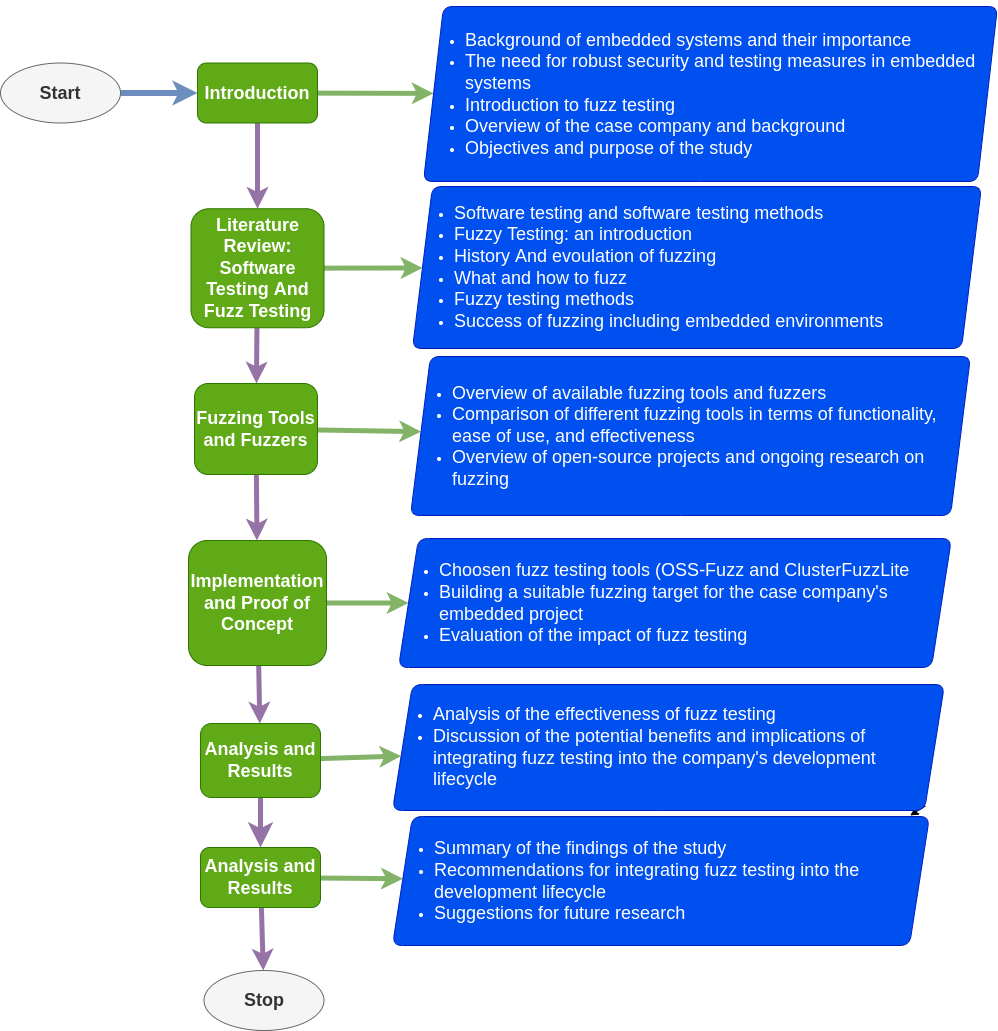
\includegraphics[width=14.5cm,height=20.4cm,keepaspectratio]{thesis_structure}}
        \caption{Thesis Flow Chart}\label{fig:thesis_structure}
\end{figure}

\clearpage